\documentclass{article}
\usepackage[utf8]{inputenc}
\usepackage{graphicx}
\usepackage{caption}
\usepackage{indentfirst}
\usepackage{pdfpages}
\usepackage{float}
\usepackage{lscape}
\usepackage{hyperref}
\hypersetup{
    colorlinks=true,
    filecolor=blue,
    citecolor=violet,
    urlcolor=blue
}
\usepackage{listings}
\usepackage[backend=biber,style=alphabetic,sorting=ynt]{biblatex}

\usepackage{enumitem,amssymb}
\newlist{todolist}{itemize}{2}
\setlist[todolist]{label=$\square$}
\usepackage{pifont}
\newcommand{\cmark}{\ding{51}}%
\newcommand{\xmark}{\ding{55}}%
\newcommand{\done}{\rlap{$\square$}{\raisebox{2pt}{\large\hspace{1pt}\cmark}}%
\hspace{-2.5pt}}
\newcommand{\wontfix}{\rlap{$\square$}{\large\hspace{1pt}\xmark}}

\addbibresource{bibliography.bib}

\setlength{\parskip}{0.4em}
        
\title{Peer-to-Peer Systems and Security \\
        \large{IN2194, SoSe 17} \\
        \huge{Onion Forwarding module} \\
        \small{for Anonymous and Unobservable VoIP Application} \\
        \bigbreak
        \large{\textbf{Final Report}}}
\author{Team \textbf{\#27} \\
\textbf{Eiler Poulsen} (03692108), Informatics (M.Sc.) \\
\textbf{Illia Ovchynnikov} (03692268), Informatics (M.Sc.)}
\date{August 2017}

\begin{document}

\null
\nointerlineskip
\vfill
\let\snewpage \newpage
\let\newpage \relax
\maketitle
\let \newpage \snewpage
\vfill 
\break

\hypersetup{linkcolor=black} % disable link highlighting for TOC
\tableofcontents
\hypersetup{linkcolor=blue}
\break

\section{Introduction}
The aim of the project is to build an Onion Forwarder module for an anonymous VoIP application using a P2P architecture.

The Onion Forwarder deals with constructing onion tunnels for tunneling data streams from UI module. At the beginning of each round the Onion Forwarder is requested to start constructing a tunnel with at least two [configurable] intermediate hops which are selected at random by querying RPS, - a Random Peer Sampler.

Tunnel building is done iteratively. A peer \textit{O} building a tunnel selects the first hop peer \textit{H\textsubscript{1}} at random, then forms an ephemeral session key \textit{K\textsubscript{1}} with the peer using external Onion Authorization module. It then uses \textit{K\textsubscript{1}} to encrypt necessary meta-data to \textit{H\textsubscript{1}} to instruct it to connect to the next hop peer \textit{H\textsubscript{2}} and establish an ephemeral session key \textit{K\textsubscript{2}}. \textit{K\textsubscript{2}} is generated by the hostkeys of \textit{O} and \textit{K\textsubscript{2}}, so that \textit{H\textsubscript{1}} does not learn about it i.e. done via Onion Routing.

Like tunnel building, data forwarding is done via Onion Routing, where datum messages are encapsulated in layers of encryption, analogous to layers of an onion. The encrypted data is transmitted through a series of network nodes, each of which "peels" away a single layer, so that The sender remains anonymous because each intermediary knows only the location of the immediately preceding and following nodes.

To reduce data diversity all P2P packages between onions are of a fixed size. Onion Forwarder also supports sending cover (fake) data so that even a MITM of a tunnel still have to overcome the dilemma whether the traffic observed is cover or real.

\section{Project Team}
The team \#27, which is responsible for the given project, consists of 2 students:

\begin{itemize}
\item \textbf{Eiler Poulsen} (03692108), Informatics (M.Sc.);
\item \textbf{Illia Ovchynnikov} (03692268), Informatics (M.Sc.).
\end{itemize}

The previous experience of the team which may be relevant to the project has purely academical nature:

\begin{itemize}
\item \textbf{Eiler} worked on a client/server version of the well-known tabletop game Battleship in Java;
\item \textbf{Illia} was engaged in a team project for a client/server service for organizing chatting conferences using vanilla Java sockets.
\end{itemize}

\section{Workload Distribution}
\textbf{Illia}'s primary responsibility and added value is core Onion Forwarding module including:
\begin{enumerate}
  \item P2P protocol design
  \item Tunnel Building (incl. incoming tunnel notification)
  \item Tunnel Retiring
  \item Data Forwarding (incl. incoming data notification)
  \item Cover (Fake data forwarding) Mechanism
\end{enumerate}

Apart from the already mentioned, \textbf{Illia} has also implemented:
\begin{enumerate}
  \item A TCP client for a RPS module
  \item Onion Forwarding In-Memory Sample, - a CLI application for demonstrating Onion Forwarder capabilities between locally deployed onions
  \item Most of the project-wide utility classes, including configurations loader from INI files.
  \item In-Memory Fakes for Onion Authorization (usese onion Base64 "encryption") used in Onion Forwarder tests and Onion Forwarding In-Memory Sample
\end{enumerate}

In addition to code related activities, \textbf{Illia} was managing such Software Configuration Management activities as Promotion \& Branch Management (repository and workflow setup), Build Management (build system setup, CI server integration) and Quality Management (code reviews, static analysis server (Circle incl. pmdcheck) integration).

Effort spent for the project: \textbf{115h}

To get to know with more detailed overview of his workload see \href{https://goo.gl/77wA6y}{Issues} and \href{https://goo.gl/NHB9hb}{Pull Requests} assigned to \textbf{Illia} or go to the next urls: \url{https://goo.gl/77wA6y} (GitHub Issues) or \url{https://goo.gl/NHB9hb} (GitHub Pull Requests).

\textbf{Eiler} was responsible for the:
\begin{enumerate}
  \item Onion Forwarder API, that exposes TCP API for CM/UI module used to communicate with Onion Forwarder, and 
  \item A TCP client for a remote Onion Authorization module, used by Onion Forwarder to enable encoding/decoding and authorization
\end{enumerate}

Among the above, Onion Forwarder API has been implemented only.

He spent time researching the course-provided testing framework to test the project's Onion Forwarding API module. However, this proved fruitless due to the framework's Gossip module relying on a remote service which was down, and thus, the RPS module could not function properly due to its reliance on the Gossip module.

Effort spent for the project: \textbf{60h}

To get to know with more detailed overview of his workload see \href{https://goo.gl/KfV9Tu}{Issues} and \href{https://goo.gl/C1nNc9}{Pull Requests} assigned to \textbf{Eiler} or go to the next urls: \url{https://goo.gl/KfV9Tu} (GitHub Issues) or \url{https://goo.gl/C1nNc9} (GitHub Pull Requests).

\section{Current State}
According to personal estimation, the project is approximately 65\% complete. While the main Onion Forwarding module is fully functional it still requires a TCP client for a remote Onion Authorization module and more in-depth integration testing of an Onion Forwarder API.

\begin{todolist}
  \item[\done] 1. Continuous Integration (Travis-CI)
  \item[\done] 2. Continuous Code Quality (Codacy (pmdcheck))
  \item[\done] 3. Code Coverage Reports (C0 \& C1)
  \item[\done] 4. Onion Forwarder
  \item[\done] 5. INI config loader
  \item[\done] 6. Remote RPS Client
  \item[\done] 7. Onion Forwarding In-Memory Sample, - a CLI application for demonstrating Onion Forwarder capabilities between locally deployed onions
  \item[\done] 8. Onion Forwarder API
  \item[\wontfix] 9. Remote Onion Authorizer Client
  \item[\wontfix] 10. CLI Module Launcher (was blocked by 8 \& 9)
  \item[\done] 11. JavaDoc documentation
\end{todolist}

\subsection{Future Work}
These are (prioritized) features and enhancements that the developers thought of, but have not yet implemented. The topics described below may be or may not be implemented in the future:
\begin{enumerate}
  \item A TCP client for a remote Onion Authorization module
  \item In-depth integration testing of an Onion Forwarding API
  \item A CLI Launcher for a standalone Onion Forwarding module
  \item Ensure an unique Onion Forwarder tunnel state per round (rebuilding tunnels for the next period)
\end{enumerate}

\section{Software Configuration Management}
\subsection{Promotion \& Branch Management}
For version control a Git VCS and GitHub development platform have been used, which allowed to perform promotion management and work with different parts of the project at the same time.

The GitHub repository is located at \href{https://github.com/wingsofovnia/p2p-group27-onion}{https://github.com/wingsofovnia/p2p-group27-onion} and is mirrored to \href{https://gitlab.lrz.de/ga74wok/p2p-group27-onion}{https://gitlab.lrz.de/ga74wok/p2p-group27-onion} as was required.

As a branch strategy, a GitHub Flow was chosen for being lightweight, simple and effective.

\begin{figure}[H]
\centering
     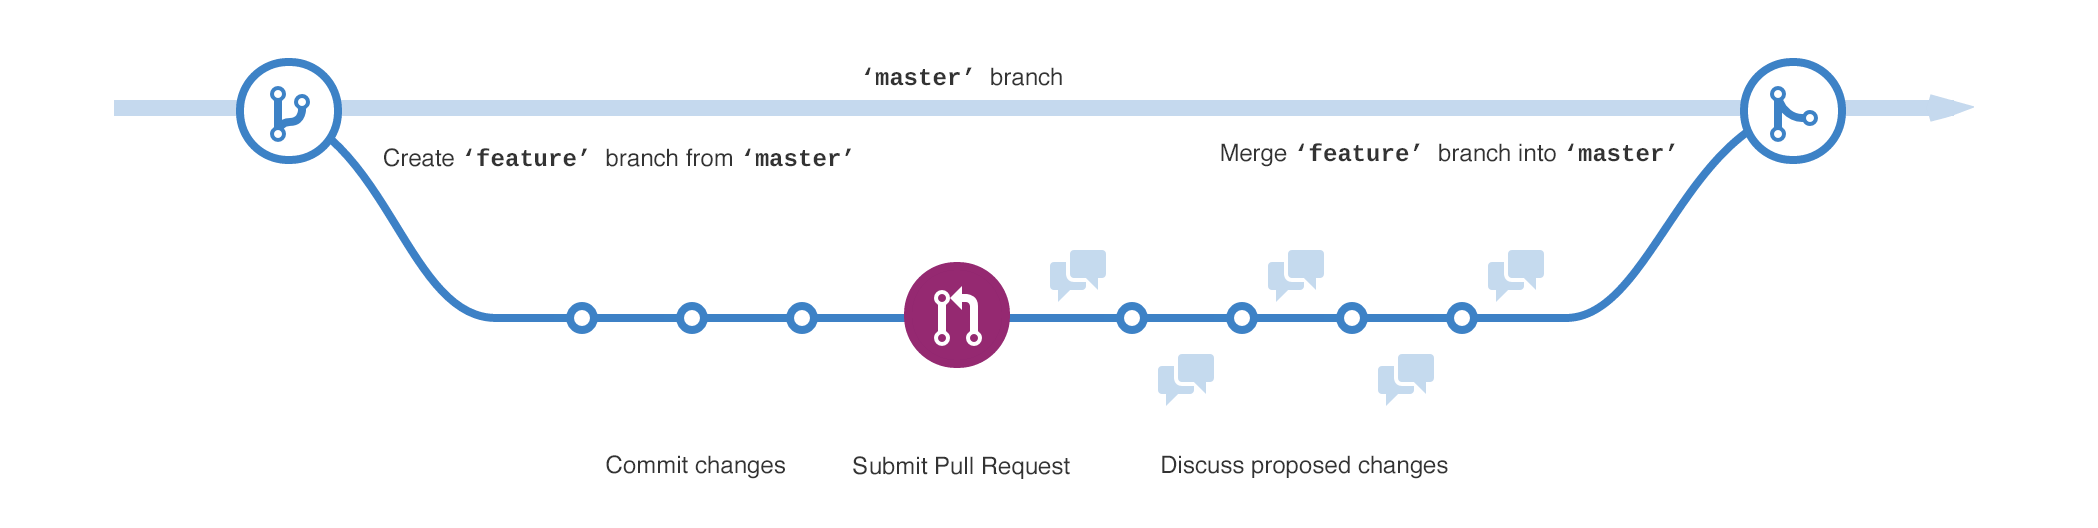
\includegraphics[width=1\textwidth]{github-flow-overview.png}
      \caption{GitHub Flow Overview \cite{githubflow}}
\end{figure}

The main rule of GitHub Flow is that master should always be deployable therefore it allows and encourages continuous delivery.

\textbf{Note!} To make commit history cleaner, the project uses a "squash merging" strategy for merging pull requests that means all commits are combined from the head branch into a single commit in the base branch. To check more detailed commit messages please have a look at corresponding pull requests. They are mentioned in each commit in the \href{https://github.com/wingsofovnia/p2p-group27-onion/commits/master}{commit log}.

\subsection{Build Management}
To manage building processes the Gradle build system has been used. It is an advanced general purpose build management system based on Groovy and Kotlin. Gradle supports the automatic download and configuration of dependencies or other libraries and allows reusing the artifacts of existing build systems.

Apart from being very flexible in terms of configuration and integration with 3-d party plugins and services, Gradle also allows adding plain old jar dependencies (like voip.jar - a testing framework) with ease that makes it of a best-fit choice for the project.

To prevent code integration problems, continuous integration server (\href{https://travis-ci.org/wingsofovnia/p2p-group27-onion}{Travis-CI}) has been used to test code integration on each promotion.

\subsection{Quality Management}
There are several strategies that has been employed to keep the quality of code as high as possible:

\begin{itemize}

\item \textbf{Code reviews} via pull requests helped the team to find mistakes overlooked in the code and ensure compliance with overall architecture and code style, improving the overall quality of software. Merges were allowed only if the build succeeds and all team's comments are resolved.

\item To ensure that previously developed and tested code still performs the same way after it was changed, continuous integration server performed \textbf{regression testing} on each promotion.

\item Equally important service in increasing software quality was \href{https://www.codacy.com/app/wingsofovnia/p2p-group27-onion}{Codacy} - an automated code review server that includes \textbf{static analysis} (includes pmdcheck) that analyzed the code for potential issues. The project was \href{https://www.codacy.com/app/wingsofovnia/p2p-group27-onion}{graded A} (being the best grade) \href{https://support.codacy.com/hc/en-us/articles/207994765-What-are-the-different-Grades-and-how-are-they-calculated-}{level} by Codacy.

\item During the work on the project, a couple of \textbf{pair programming sessions} and walkthroughs ocurred. They allowed to overcome complex tasks faster, increased the level of productivity and the quality of the code.
\end{itemize}

\section{Documentation}

\subsection{Programming Language and Target Platforms}
The software solution is written in Java. The arguments in favor are mostly due to team's familiarly with the language and its stack. There is also a vast array of libraries available and a lot of supportive documentation on how to design and develop network applications.

Generally speaking, the software solution is likely run on all platforms that can run Oracle JRE (Java Runtime Environment) version 1.8 (tested on update \#112 and up), however, Windows 10 and MacOS Sierra are the only directly supported platforms targeted as they are team's development environment of choice.

The project includes Gradle wrapper and so that a standalone Gradle installation to build or run the app is not required.

\subsection{Javadoc}
Most classes and methods are comprehensively documented with JavaDoc. The documentation can be generated by running Gradle \verb|javadocs| task. Documentation will be available at \verb|build/docs/javadoc/index.html| then.
\begin{lstlisting}
$ ./gradlew clean javadocs
\end{lstlisting}

Whereas Windows users should use \verb|gradlew.bat| wrapper to generate documentation:
\begin{lstlisting}
> gradlew.bat clean javadocs
\end{lstlisting}

\subsection{Architecture}

\subsubsection{Overview}
A backbone of the implemented Onion Forwarding module is a Netty I/O framework with a well-defined event model based on Interceptor Chain Pattern.

In Netty, all incoming requests are intercepted by a single thread (the Selector), queued, and subsequently processed asynchronously by threads (Thread Handlers) from a thread pool.

\begin{figure}[H]
\centering
     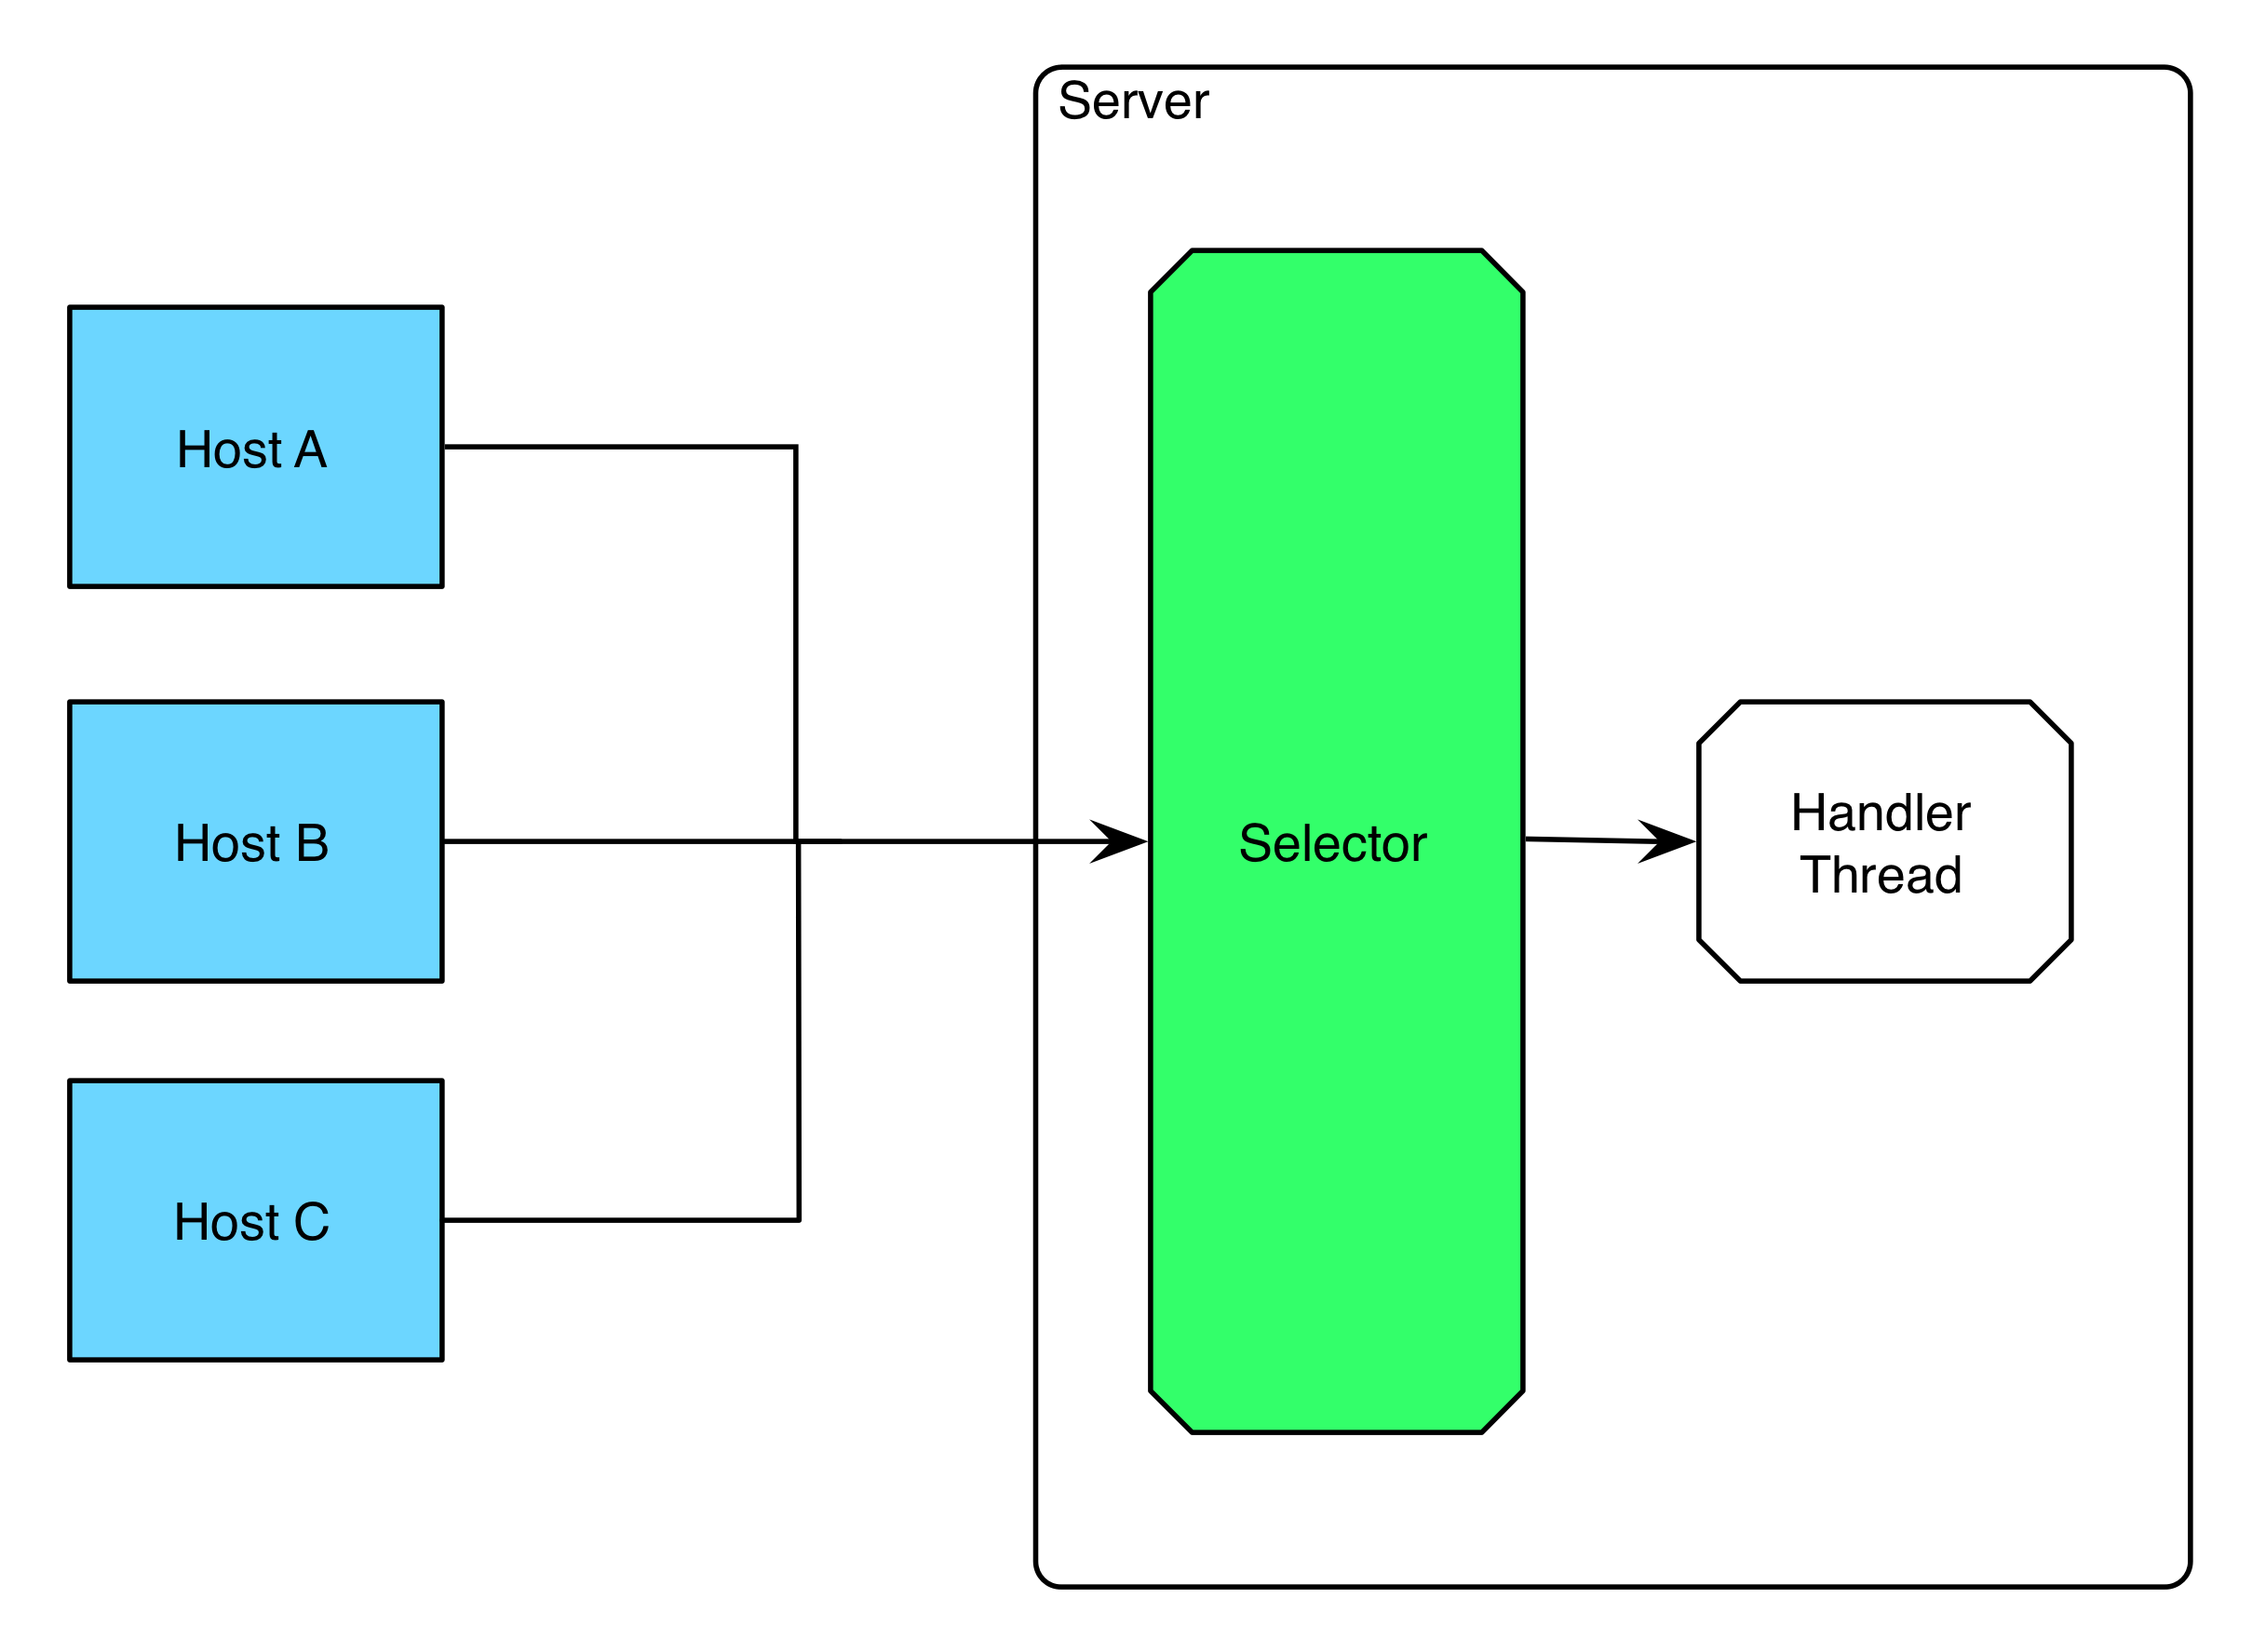
\includegraphics[width=0.7\textwidth]{netty-req-quering.png}
      \caption{Illustration of Netty's I/O architecture \cite{netty}}
\end{figure}

Netty introduces a concept of pipelines for events in which a task can be sequentially processed in multiple steps. This is a powerful concept considering the application in question and the data being transported; layered packaged data that must be and processed in multiple steps.

\begin{figure}[H]
\centering
     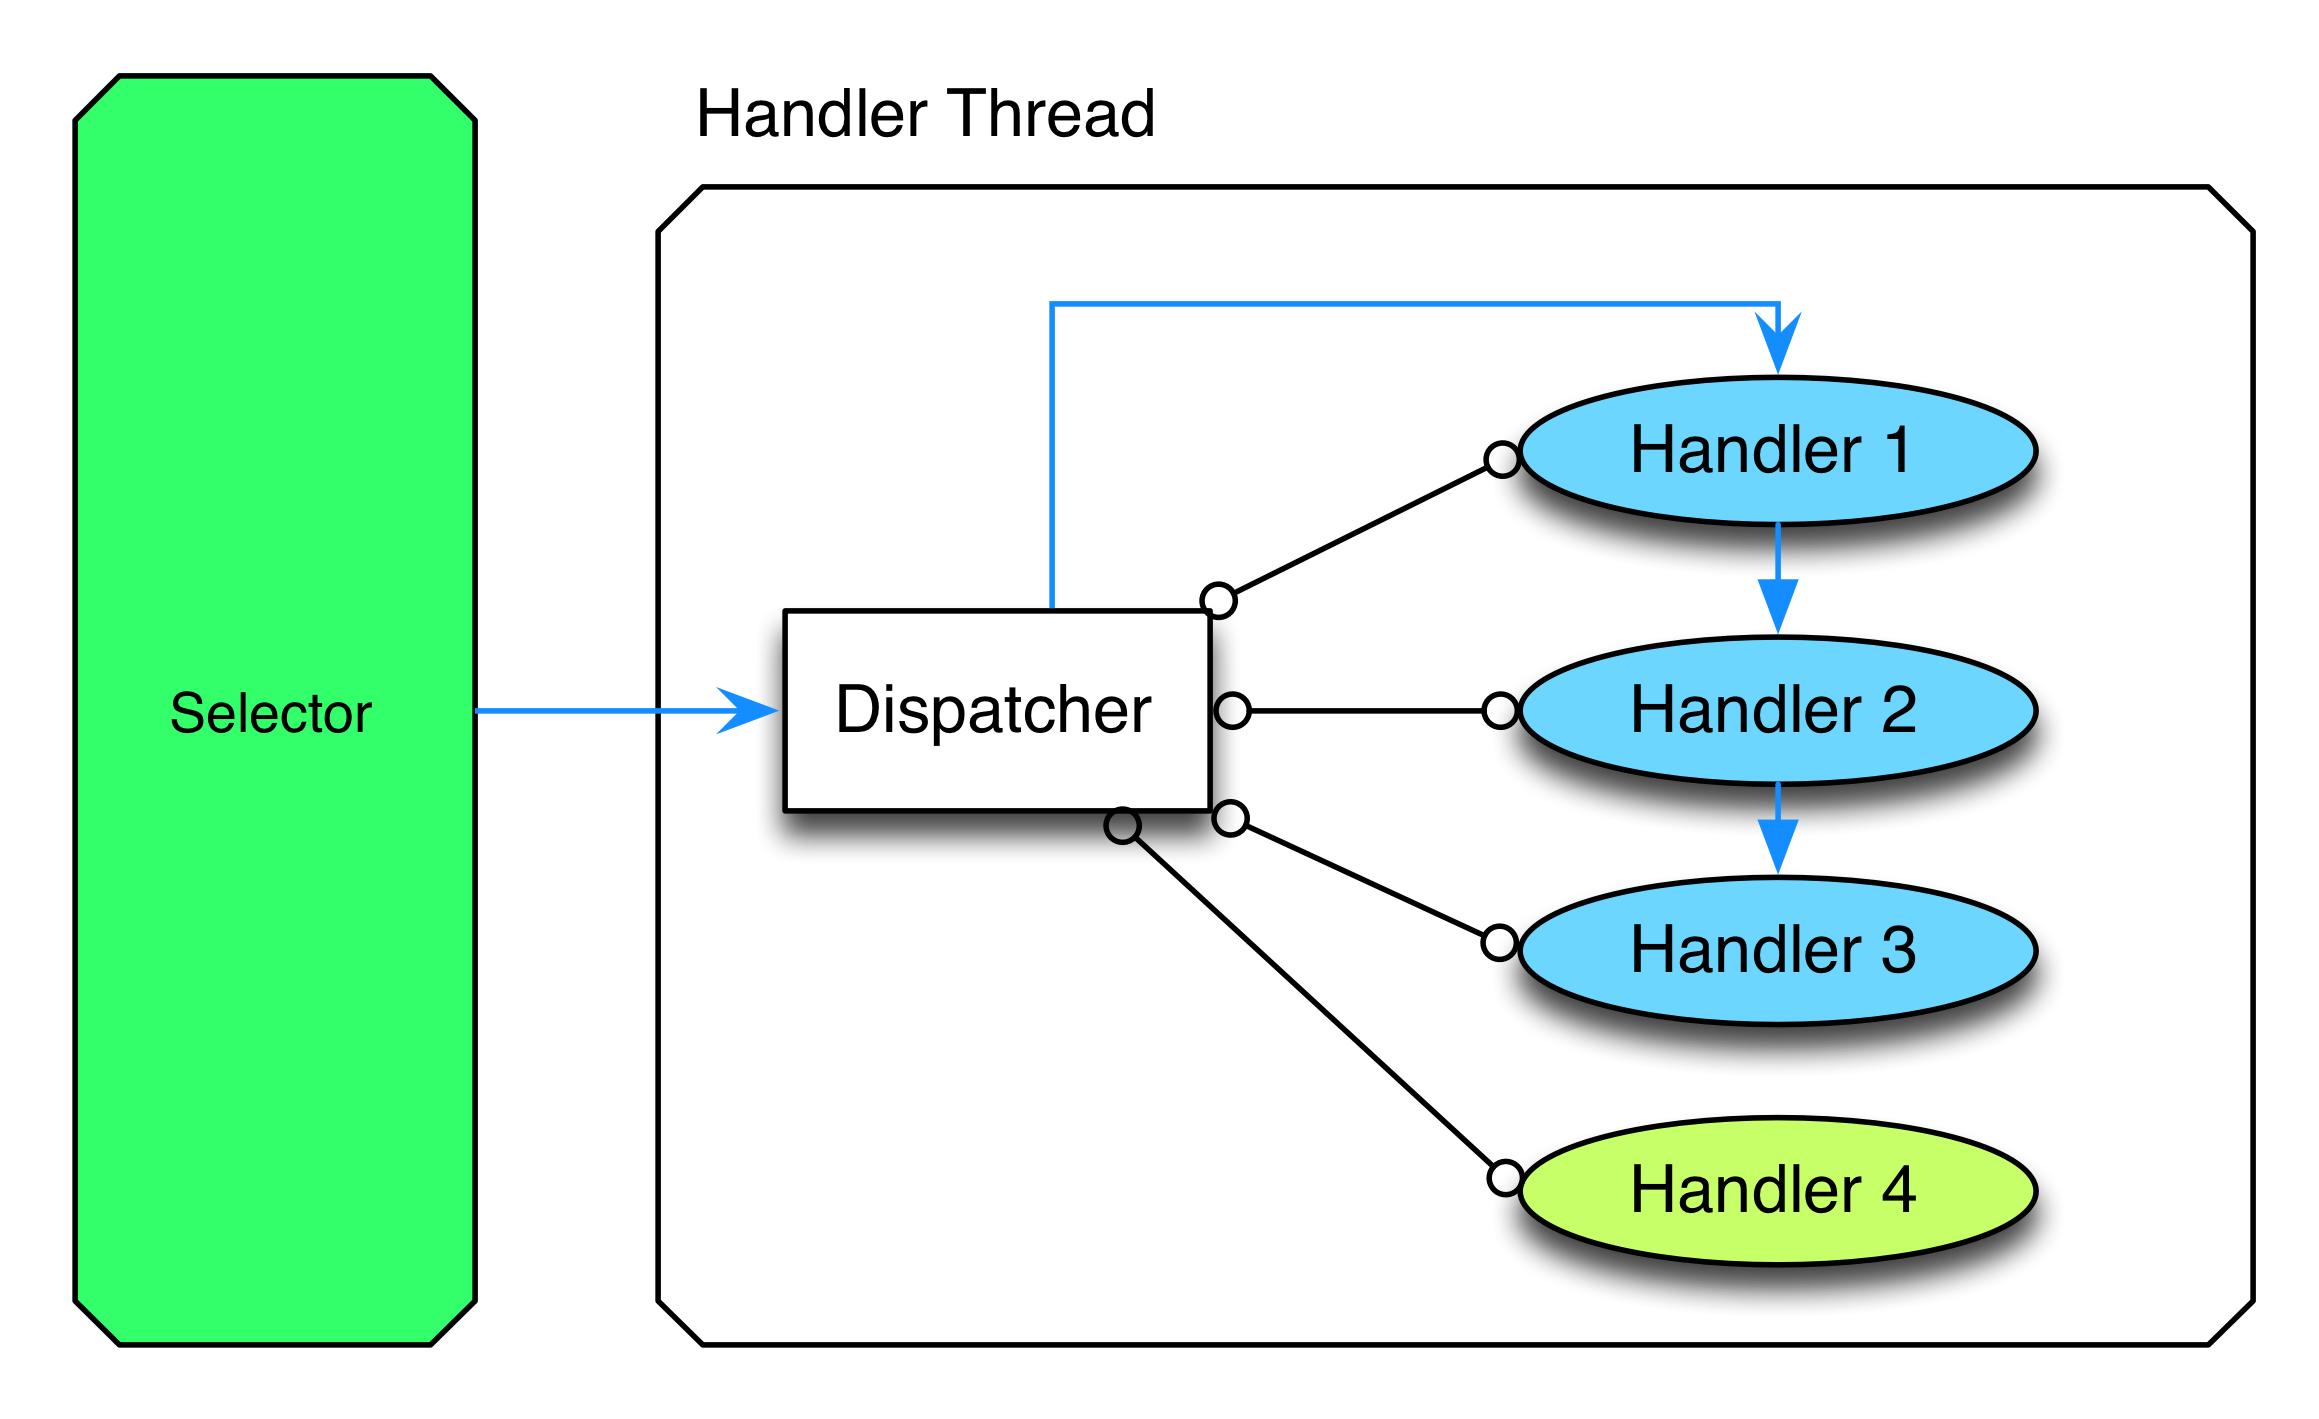
\includegraphics[width=0.7\textwidth]{netty-handlers-chain.png}
      \caption{Netty Interceptor Chain Pattern implementation for handlers \cite{netty}}
\end{figure}

Netty also provides build-in handlers for length prefix framing, fixed length frame decoders that are required for the protocols defined for the API and P2P communication respectively. 

The end result is a secure, non-blocking, high performant and scalable solution by design.

The Onion Forwarding module is mainly represented by the following components:

\begin{enumerate}
  \item \textbf{OnionForwarder} is responsible for forwarding data between API connections and Onion Tunnels.
  \begin{itemize}
    \item \textbf{OnionForwarderAPI} exposes TCP API for CM/UI module used to communicate with Onion Forwardining.
  \end{itemize}
  \item \textbf{OnionAuthorizer} encapsulates authentication and encryption mechanisms used while building onion tunnels. It implements establishing session keys given hostkeys of hops, and onion layer-encryption and decryption of payload data.
  \begin{itemize}
    \item \textbf{SessionFactory} encapsulates Diffie–Hellman key exchange flow specific for Onion Auth specification.
  \end{itemize}
  \item \textbf{RandomPeerSampler} is geared towards helping find peers at random.
\end{enumerate}

%\begin{landscape}
\begin{figure}[H]
\centering
  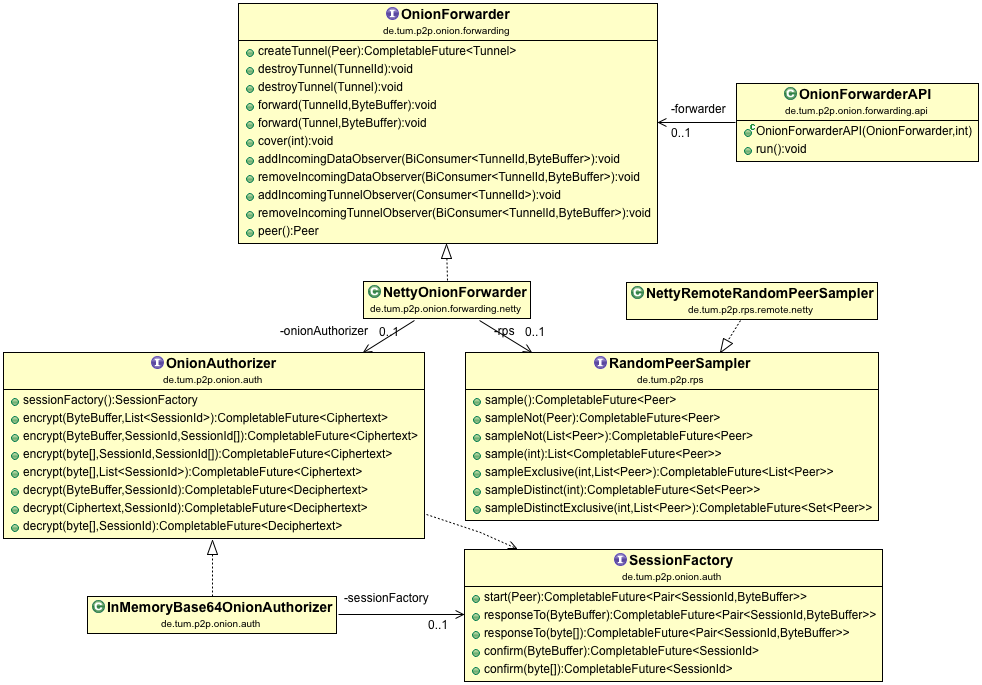
\includegraphics[angle=90,height=1.45\textwidth]{cd-onion-fwd-auth-rps.png}
  \captionsetup{justification=centering}
  \caption{UML Class Diagram of the most significant components of the Onion Forwarding module}
\end{figure}
%\end{landscape}

Such separation allowed not only to encourage single responsibility principle but also allows more granular workload distribution.

Each Onion holds at least one server socket connection and may hold multiple client socket which point to next or prev onion's server the onion should route data messages. For example, the onion, that is an originator O(1) of a tunnel connection will hold 2 connections - bind (server) and client connection to the next hop O(2):
\begin{figure}[H]
\centering
     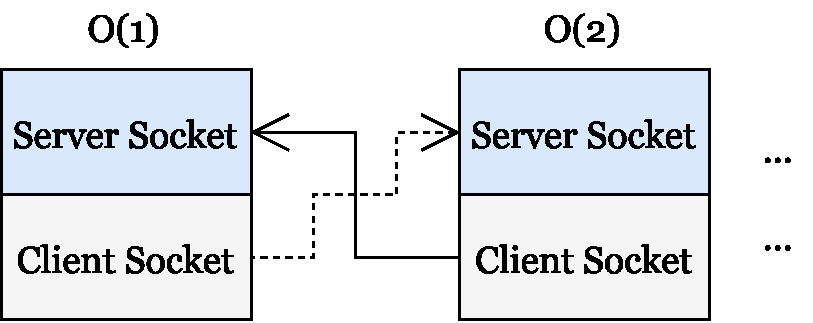
\includegraphics[width=0.5\textwidth]{onion-sockets-connections.pdf}
      \caption{Onion P2P Socket Connections}
\end{figure}

The onion's server pipeline consists of the following handlers:
\begin{enumerate}
  \item \textbf{FixedLengthFrameDecoder} (inbound) splits the received data stream by the fixed number of bytes that corresponds to a size of single message of a onion P2P protocol.
  \item \textbf{TunnelRetireHandler} (inbound) handles TUNNEL RETIRE messages and clears routing context from routes assigned to tunnel id given in the message.
  \item \textbf{TunnelRelayHandler} (inbound) performs onion decryption of a payload of TUNNEL RELAY message. As soon as the last layer is peeled out, the payload is extracted and propagated down the Netty's pipeline so further handlers can process payloads separately.
  \item \textbf{TunnelConnectHandler} (inbound) receives TUNNEL CONNECT payloads propagated from TunnelRelayHandler, creates a TUNNEL EXTEND message, connects to the peer to be a new member of the tunnel and forwards the extend request.
  \item \textbf{TunnelExtendHandler} (inbound) handles incoming TUNNEL EXTEND message received by the onion that is requested to be a new peer in the tunnel. The handler generates HS2, forms a TUNNEL EXTENDED message and propagates the message up the tunnel.
  \item \textbf{TunnelDatumHandler} (inbound) handles plaintext TUNNEL DATUM messages received from unwrapping TUNNEL RELAY message by TunnelRelayHandler. It checks whether the datum is cover or not and then notify OnionForwarder's data listeners.
  \item \textbf{TunnelMessageDecoder} (inbound) decodes TUNNEL * messages from bytes to corresponding internal message type.
  \item \textbf{TunnelMessageEncoder} (outbound) encodes all outcoming internal messages to bytes.
\end{enumerate}

The client pipeline is relatively simple and consists of several handlers:
\begin{enumerate}
  \item \textbf{FixedLengthFrameDecoder} (inbound) splits the received data stream by the fixed number of bytes that corresponds to a size of single message of a onion P2P protocol.
  \item \textbf{TunnelExtendedHandler} (inbound) handles TUNNEL EXTENDED messages and make sure the message arrive to the first peer which will complete tunnel extension, i.e. the handler will propagate the message up the tunnel till there is a prev hop in a routing context.
  \item \textbf{TunnelMessageDecoder} (inbound) decodes TUNNEL * messages from bytes to corresponding internal message type.
  \item \textbf{TunnelMessageEncoder} (outbound) encodes all outcoming internal messages to bytes.
\end{enumerate}

\subsubsection{Protocol}

Onion-to-onion communication is done via packages of fixed 1024 bytes size (configurable by constant) and automatic padding with random bytes therefore such packages do not require length prefix framing.

An origin onion \textit{O} constructs tunnels incrementally, negotiating a symmetric key with each peer on the tunnel, one hop at a time. To begin creating a new tunnel, the \textit{O} sends a Tunnel Extend request to the first hop peer \textit{H\textsubscript{1}} in its chosen path. The message's payload contains the first half of the Diffie-Hellman handshake and a hostkey of the \textit{O}.

\begin{figure}[H]
\centering
     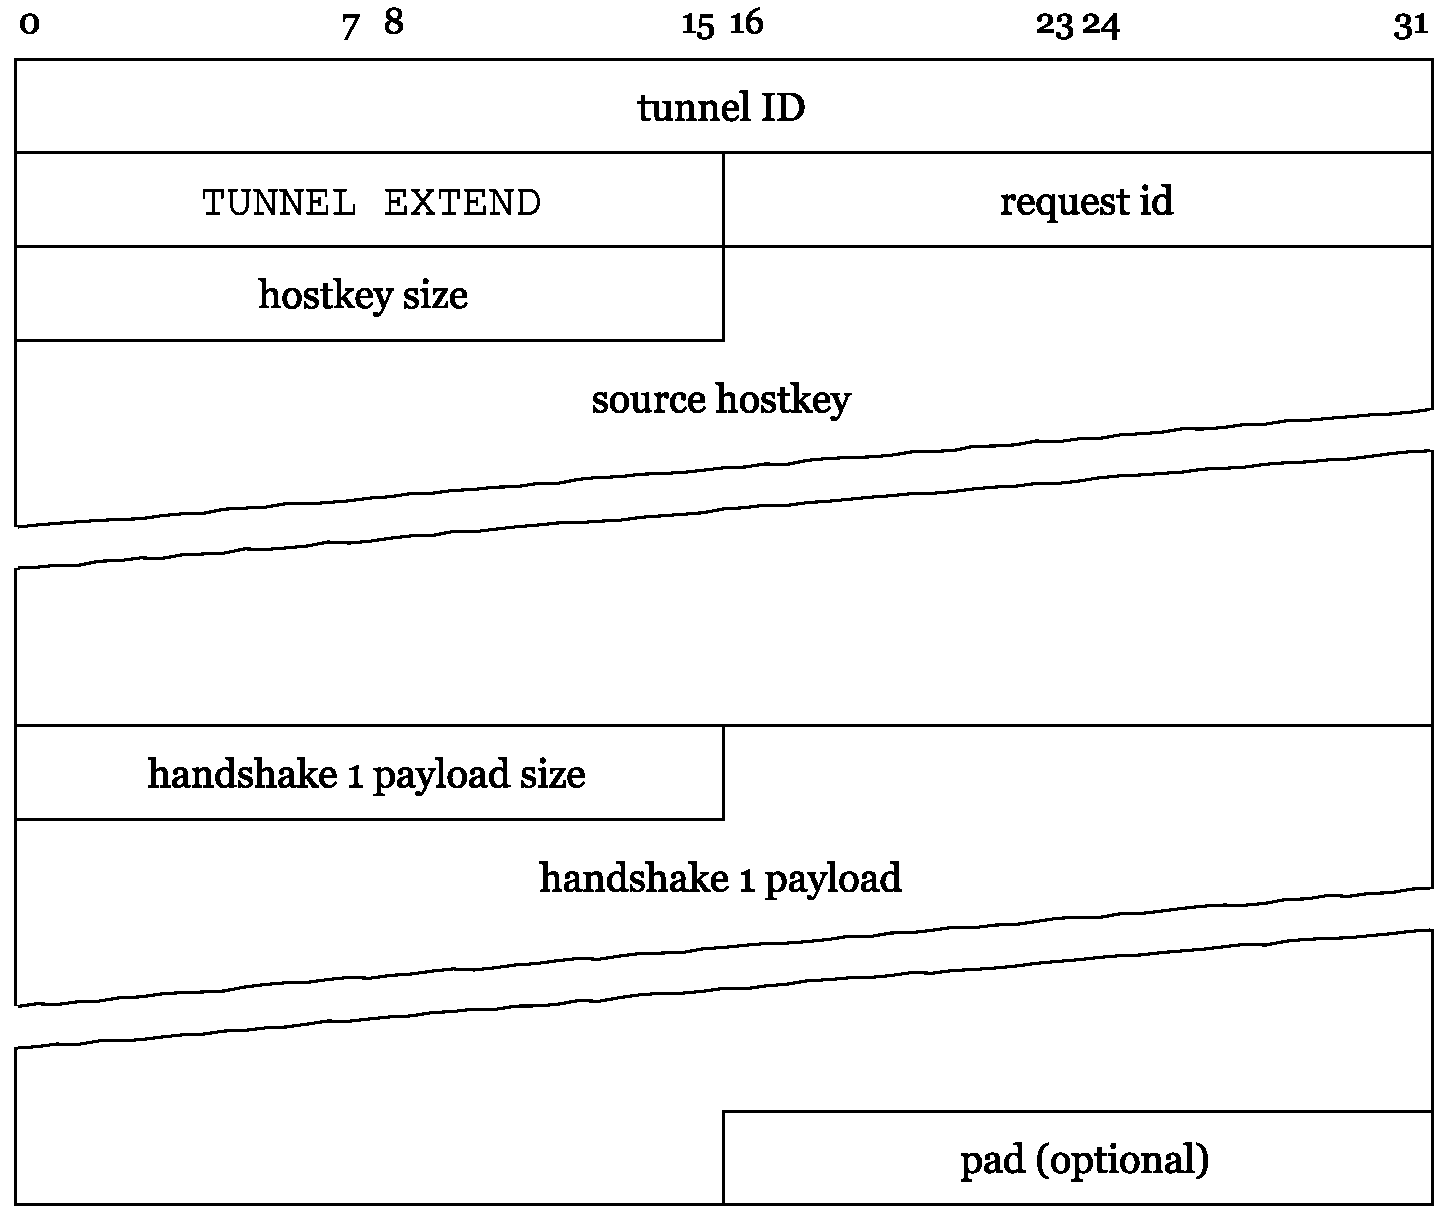
\includegraphics[width=0.75\textwidth]{tunnel-extend.pdf}
      \caption{Tunnel Extend protocol data unit}
\end{figure}

\textit{H\textsubscript{1}} then responds with a Tunnel Extended message containing the second half of the Diffie-Hellman handshake.
\begin{figure}[H]
\centering
     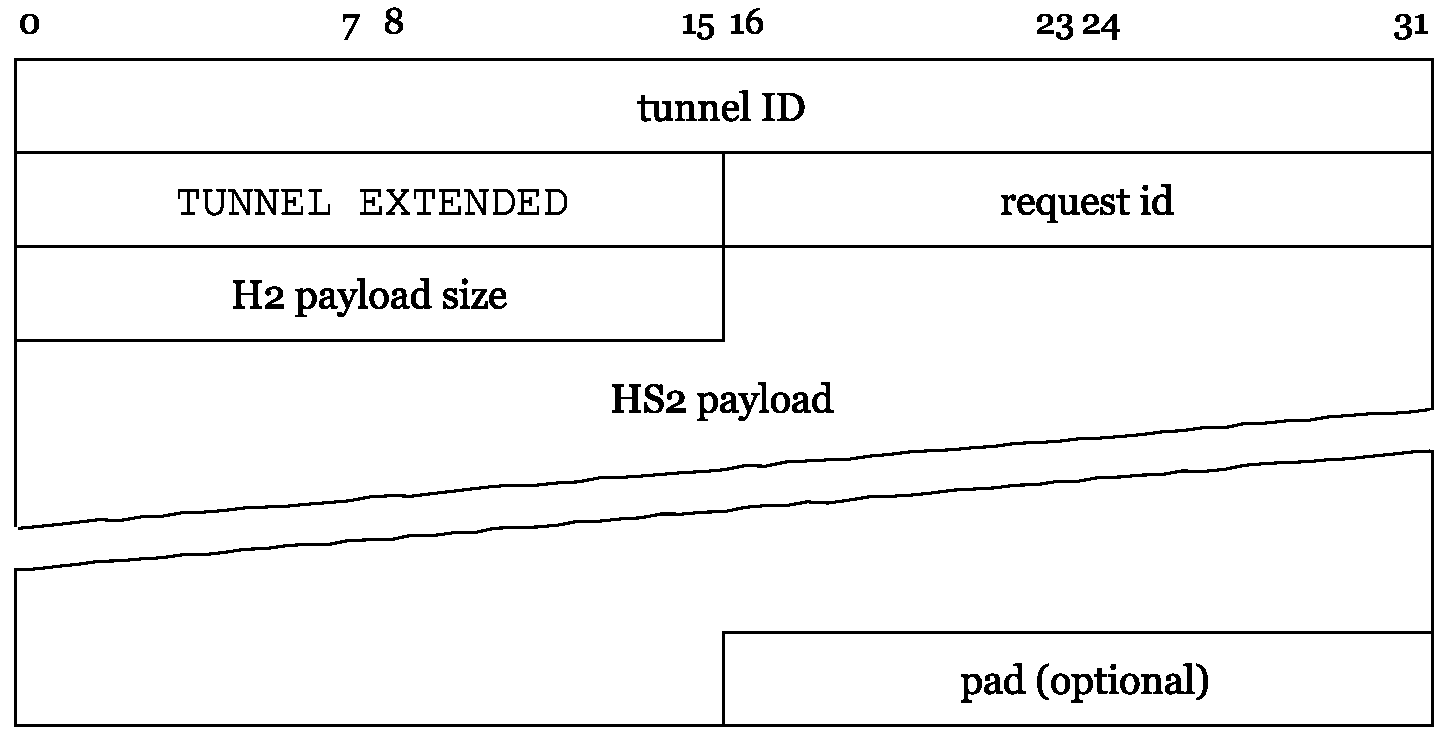
\includegraphics[width=0.75\textwidth]{tunnel-extended.pdf}
      \caption{Tunnel Extended protocol data unit}
\end{figure}

Once the tunnel has been established, \textit{O} and \textit{H\textsubscript{1}} can communicate securely with the negotiated key \textit{K\textsubscript{1}}.

Tunnel Relay is a container for encrypted payloads that are peeled out on each round of tunnel building or datum forwarding. Tunnel Relay's payload can be either Tunnel Connect or Tunnel Datum.
\begin{figure}[H]
\centering
     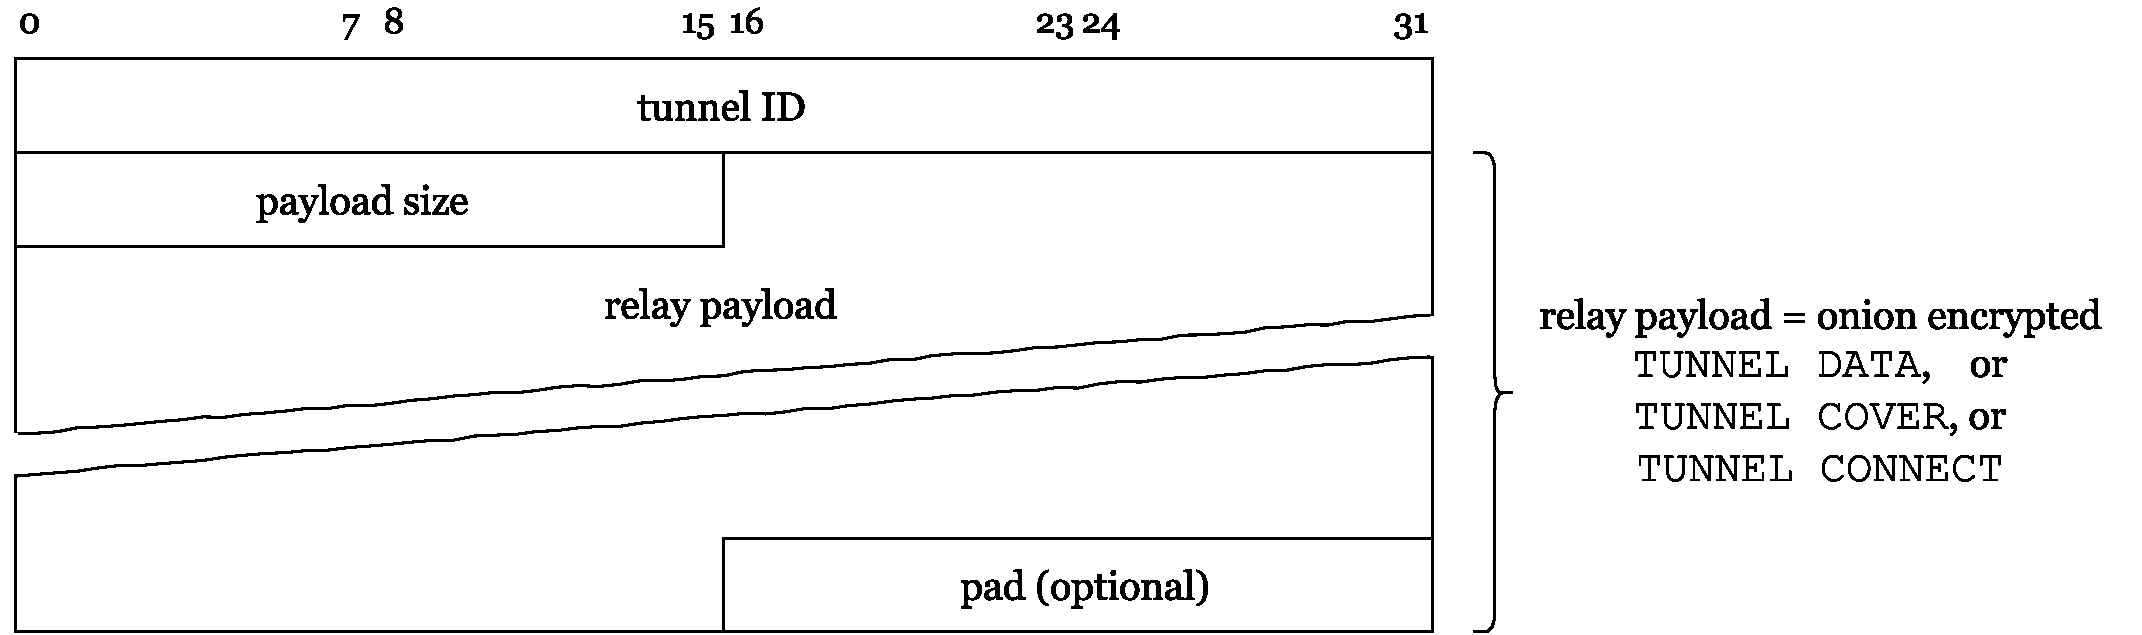
\includegraphics[width=1\textwidth]{tunnel-relay.pdf}
      \caption{Tunnel Relay protocol data unit}
\end{figure}

Upon receiving a Tunnel Relay message, each onion is responsible for peeling out a layer of encrypted payload with its session key and passing the Tunnel Relay down the tunnel.

To extend the tunnel further, \textit{O} iteratively sends onion encrypted Tunnel Connect requests that are carried by Tunnel Relay. The last onion in the tunnel \textit{H\textsubscript{N-1}} is then required to decrypt the last layer of encryption, copy the half-handshake into a new Tunnel Extend message and pass it to \textit{H\textsubscript{N}} to extend the tunnel. 

\begin{figure}[H]
\centering
  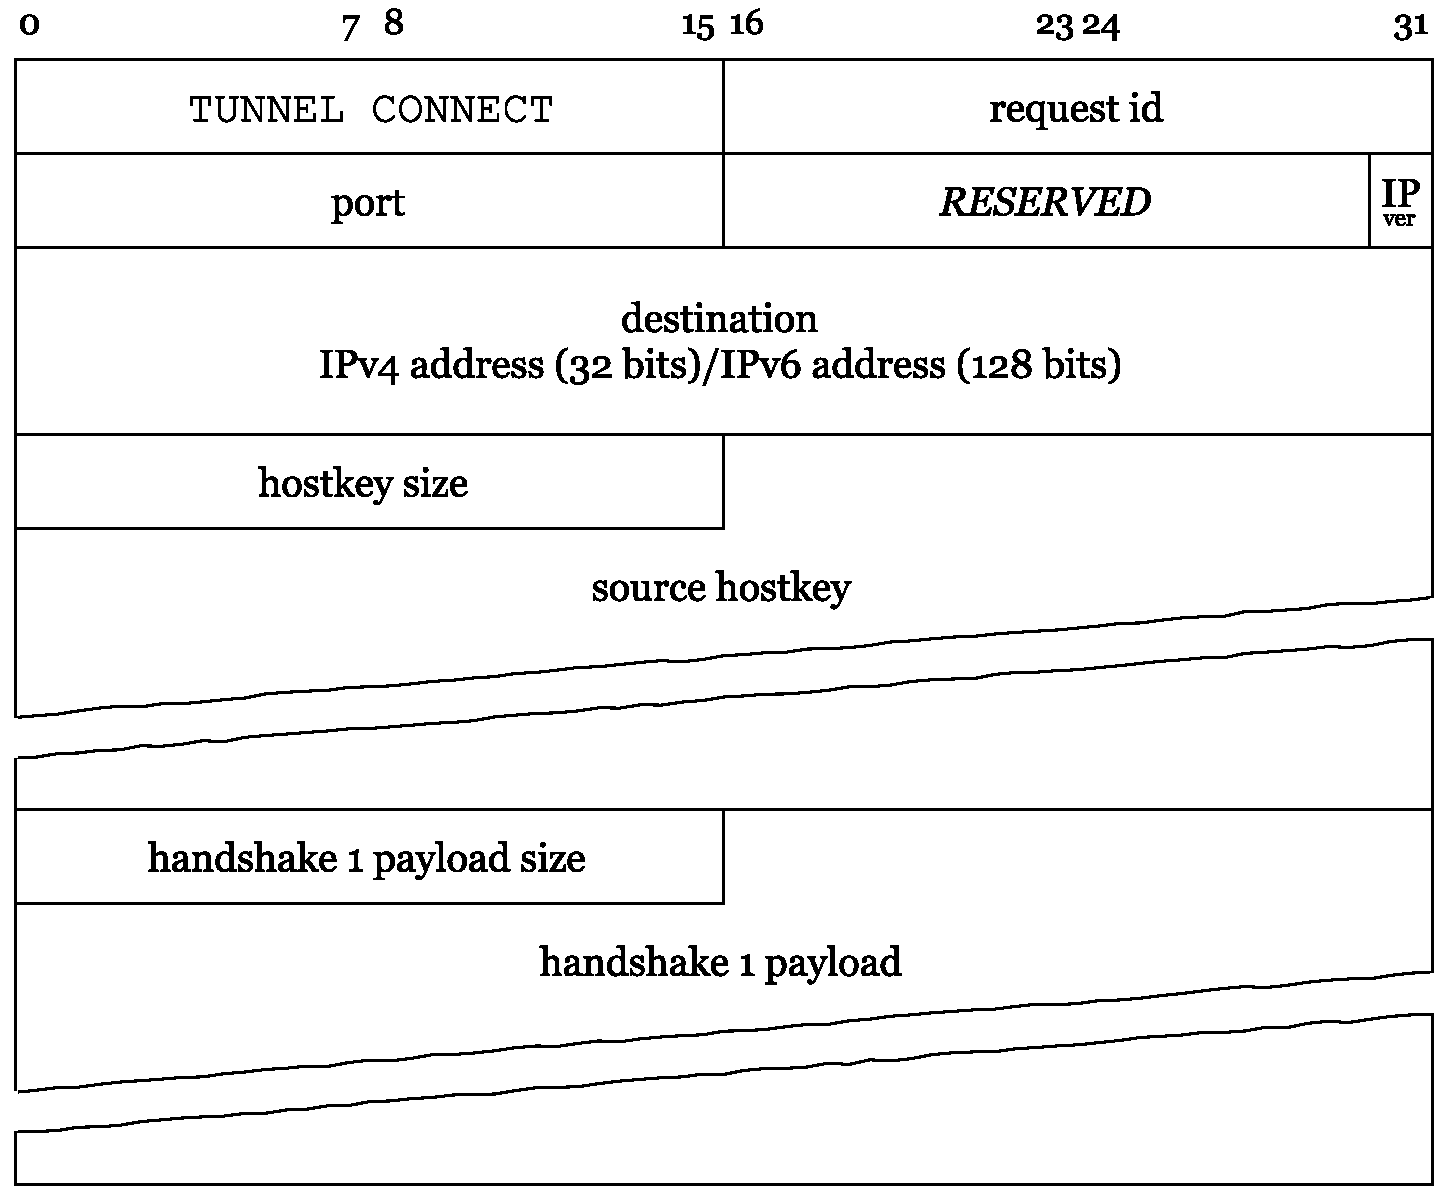
\includegraphics[width=0.8\textwidth]{tunnel-connect.pdf}
  \captionsetup{justification=centering}
  \caption{Tunnel Connect protocol data unit and payload of the Tunnel Relay protocol data unit}
\end{figure}

\textit{H\textsubscript{N}} responses then with Tunnel Extended message that is propagated up the tunnel to the first onion \textit{O}.

Once \textit{O} has established the tunnel it can relay data in Tunnel  Datum messages. These messages are onion encrypted and carried by Tunnel Relay just like Tunnel Connect requests.

\begin{figure}[H]
\centering
     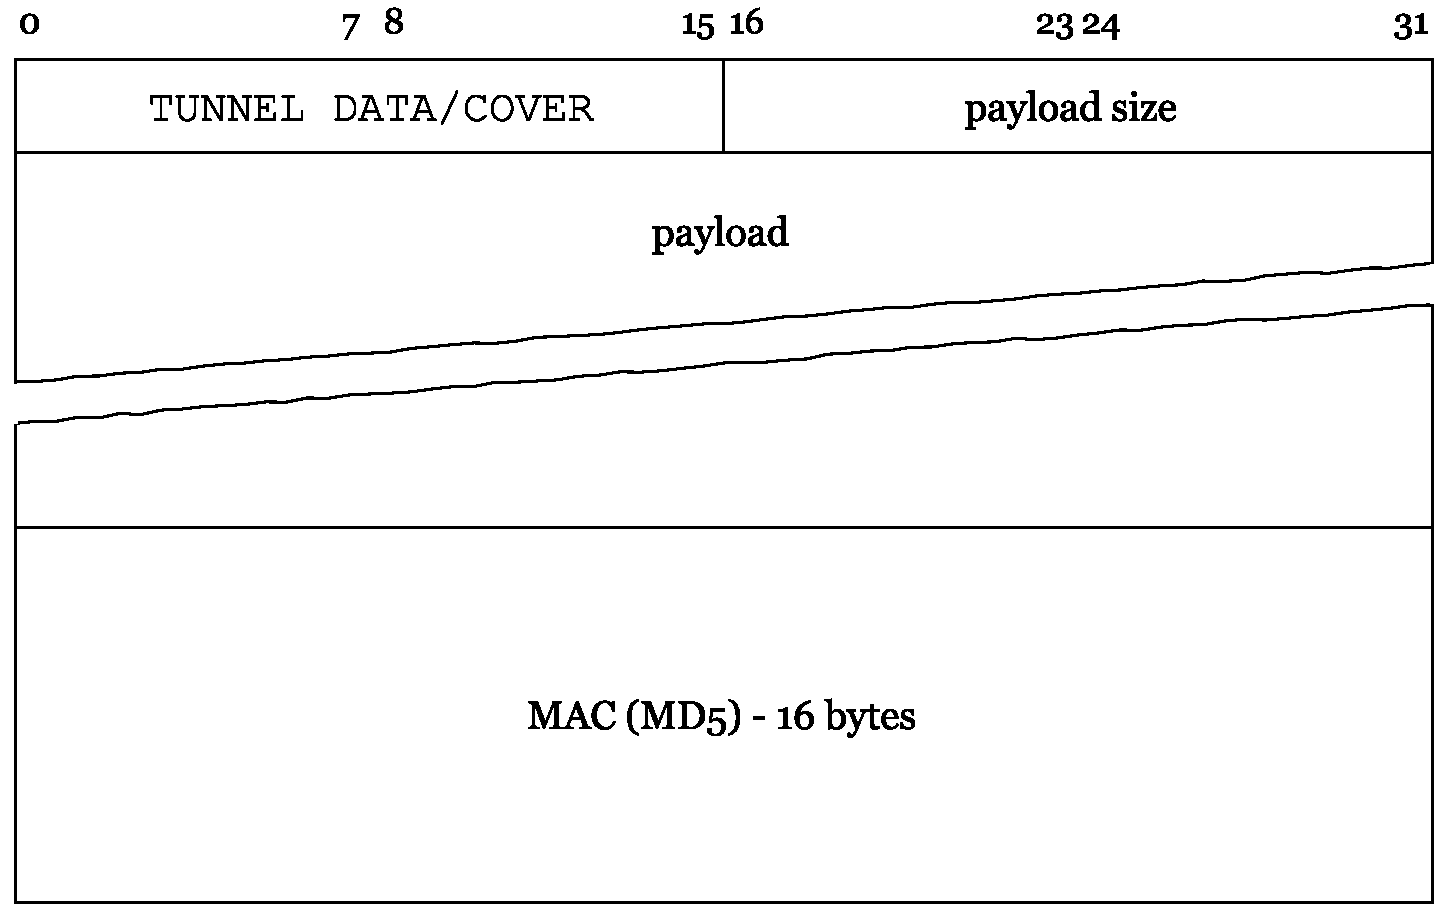
\includegraphics[width=0.8\textwidth]{tunnel-datum.pdf}
      \caption{Tunnel Data payload of the Tunnel Relay protocol data unit}
\end{figure}

This protocol data unit is used for cover data also, only PDU message type header changes to Tunnel Cover. Since the payload is onion encrypted (including the msg type header) a potential attacker has no idea whether the message is fake or not.

To enable confidentiality, integrity, and authenticity (Authenticated Encryption) message contains message authentication code generated using Encrypt-then-MAC scheme.

To tear down a tunnel, \textit{O} sends a Tunnel Retire message. The \textit{H\textsubscript{1}} onion receives the message, tear down all resources associated with this tunnel and propagates the message down the tunnel to further peers.

\begin{figure}[H]
\centering
     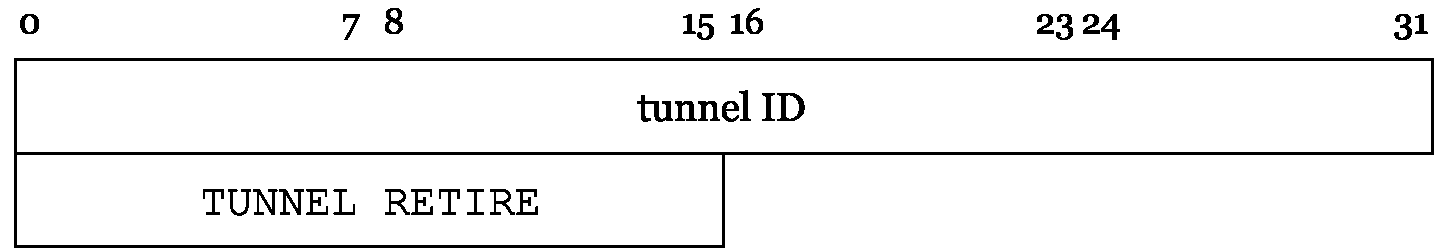
\includegraphics[width=0.75\textwidth]{tunnel-retire.pdf}
      \caption{Tunnel Retire protocol data unit}
\end{figure}

\subsection{Build the Project}
To build the project it's required to run Gradle \verb|assemble| task. The project includes Gradle wrapper \verb|gradlew| and so that a standalone Gradle installation to build or run the app is not required.
\begin{lstlisting}
$ git clone \ 
     https://github.com/wingsofovnia/p2p-group27-onion.git
$ cd p2p-group27-onion

$ ./gradlew clean assemble
\end{lstlisting}

Whereas Windows users should use \verb|gradlew.bat| wrapper to build the project:
\begin{lstlisting}
> gradlew.bat clean assemble
\end{lstlisting}

\subsection{Run Example Application}
Despite the implemented Onion Forwarding module lacks a client for a remote Onion Authorization module that is required for running standalone module as a part for the voip application, there is an example of Onion Forward implementation which can be run locally to demonstrate data forwarding without required remote Onion Authorizer and RPS. All onion are run locally with in-memory Onion Authorizer and RPS fakes.

To run the example please follow these steps:
\begin{enumerate}
  \item Compile the project
    \begin{lstlisting}
$ ./gradlew clean jar
    \end{lstlisting}
  \item Run example
  \begin{lstlisting}
$ java -jar samples/build/libs/onion-f...SNAPSHOT.jar
    \end{lstlisting}
  \item It's also possible to parametrize the amount of local onions by passing it as an argument. For example, to run the example with 4 local onions:
  \begin{lstlisting}
$ java -jar samples/build/libs/onion...SNAPSHOT.jar 4
    \end{lstlisting}
\end{enumerate}

Example output of the example app with 3 onions forwarding "test" message from onion \verb|localhost:16453| to \verb|localhost:39516|:
\begin{lstlisting}
$ java -jar samples/build/libs/onion-for...SNAPSHOT.jar 3
Number of local onions = 3
Random local peers = 
localhost:16453, 
localhost:6247, 
localhost:39516

Please select origin onion to build a tunnel
0) localhost:16453
1) localhost:6247
2) localhost:39516
Type: 0

Please select destination onion to build a tunnel
1) localhost:6247
2) localhost:39516
Type: 2

Building the tunnel ...
!Listener: Onion (localhost:39516) inc. tunnel #9091564
Tunnel #9091564 has been successfully built

Feel free to type any string to forward it from the 
(localhost:16453) -> (localhost:39516). 
Type 'exit' to exit.

> test
Sending "test" from (localhost:16453) to (localhost:39516) 
via tunnel #9091564

!Listener: Datum "test" arrived to (localhost:39516) 
via tunnel #9091564

> exit
Closing onions ...
$ ...
\end{lstlisting}

\subsection{Code Coverage}
Gradle \verb|check jacocoTestReport| tasks can be used to check project C0 \& C1 coverage percentage and generate a Jacoco report. Coverage statistics will be displayed after running tests and the report will be available at \verb|build/reports/jacoco/test/html/index.html|.
\begin{lstlisting}
$ ./gradlew clean check jacocoTestReport
....
BUILD SUCCESSFUL
Total time: 14.324 secs
Coverage summary:
onion-forwarding:  61,2%
\end{lstlisting}

Whereas Windows users should use \verb|gradlew.bat| wrapper:
\begin{lstlisting}
> gradlew.bat clean check jacocoTestReport
\end{lstlisting}

\section{License}
The project is distributed under the MIT license, since the purpose of this project is purely academical therefore the team decided to keep the project open source with the only requirement to keep the team's copyright notice intact when its recipients repurpose, redistribute, or otherwise reuse the code and the MIT license fulfills this requirement entirely.

%\medskip
 
\nocite{torproject}
\nocite{netty}
\nocite{onionrouting}

\printbibliography
\end{document}
